\documentclass{beamer}


\usetheme{AnnArbor}
\usecolortheme{default}


\title{Problem Solving and Creativity}
%\subtitle{Complex Systems Engineering}
\author{Steve Mazza}
\institute[Naval Postgraduate School]
{ 
    Naval Postgraduate School \\
    Monterey, CA \\
    
\includegraphics[height=3cm]{images/NPS_logo.jpg}
}
\date {SE4920, Summer/2014}
\subject{Reverse Engineering}


\begin{document}

\frame{\titlepage}


\frame{{Introduction}
  We will\dots
  \begin{itemize}
    \item Briefly discuss some ideas about problem solving
    \item Compare novice and expert problem solvers
    \item Propose a strategy for problem solving
    \item Discuss teaching problem solving
    \item Discuss creativity
  \end{itemize}
}

\frame{{Overview Of Problem Solving}
  \centering{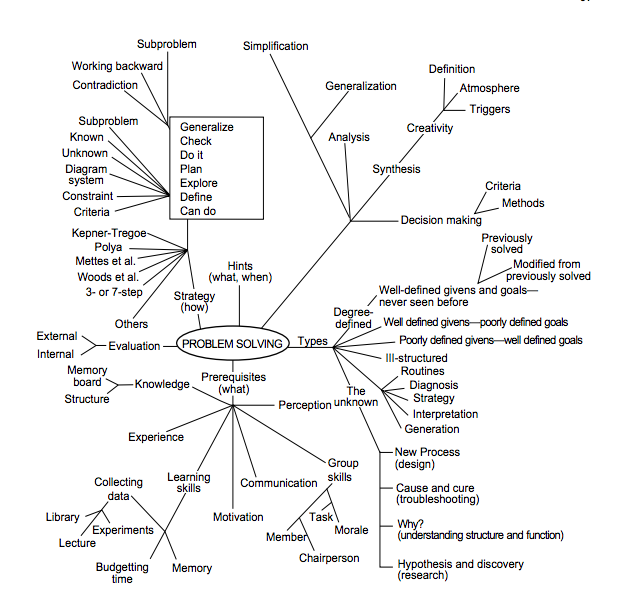
\includegraphics[scale=0.35]{images/problem.png}}
}

\frame{{Novice vs. Expert}
  \framesubtitle{Differences}
  \scriptsize
  \begin{tabular}[h]{lll}
    \hline \\
    \textbf{Characteristic} & \textbf{Novices} & \textbf{Experts} \\
    \hline \\
    Memory & Small pieces, few items & Chunks or patterns, 50,000 items \\
    Attitude & Try once and then give up & Persistent, confident \\
    Categorize & Superficial details & Fundamentals \\
    Problem statement & Inaccurate & May redefine several times \\
    Simple problems & Work backward & Work forward with known procedures \\
    Strategy & Trial and error & Known strategy \\
    Information & Don't know what is relevant & Recognize and draw inferences \\
    Parts & Does not analyze parts & Proceed in steps, look for patterns \\
    Sketching & Not done & Considerable time here \\
    \hline
  \end{tabular}
}

\frame{{Novice vs. Expert}
  \framesubtitle{Differences (continued)}
  \scriptsize
  \begin{tabular}[h]{lll}
    \hline \\
    \textbf{Characteristic} & \textbf{Novices} & \textbf{Experts} \\
    \hline \\
    Limits & Do not calculate & May use to bound solution \\
    Equations & Memorize or look up & Use fundamental relations to derive \\
    Solution procedures & Uncomplicated & Equation and solution method are same \\
    Monitoring progress & Does not & Checks off versus strategy \\
    If suck & Guess, quit & Use heuristics, persevere \\
    Accuracy & Not concerned & Very accurate, check results \\
    Evaluation of result & None & From broad experience \\
    Mistakes & Ignore & Learn, adapt \\
    Actions & Sit and think & Sketch, subvocalize \\
    Decisions & No clear criteria & Understands decision process \\
    \hline
  \end{tabular}
}

\frame{{Problem Solving Strategies}
  \begin{enumerate}
    \setcounter{enumi}{-1}
    \item I can
    \item Define
    \item Explore
    \item Plan
    \item Execute
    \item Check
    \item Generalize
  \end{enumerate}
}

\frame{{Getting Started Or Unstuck}
  \framesubtitle{Heuristics}
  \begin{enumerate}
    \item Simplify the problem and solve limiting cases.
    \item Check for under/over simplification.
    \item Relate the problem to something familiar.
    \item Generalize the problem.
    \item Try substituting in numbers.
    \item Try solving for ratios.
    \item Be sure there actually is a problem.
    \item Change the representation of the problem.
    \item Ask questions about the problem.
    \item Concentrate on the parts of the problem that can be solved.
  \end{enumerate}
} 

\frame{{Getting Started Or Unstuck}
  \framesubtitle{Heuristics (continued)}
  \begin{enumerate}
    \setcounter{enumi}{10}
    \item Be a good listener and maintain group harmony.
    \item Use a plus-minus-intersecting (PMI) approach when presented with possible solutions.
    \item Use a mixed scanning strategy.
    \item Alternate working forward and backward.
    \item Take a break.
    \item Seek hidden assumptions and look for what you forgot to use.
    \item Apply a control strategy.
    \begin{enumerate}
      \item What are you doing?
      \item Why are you doing it?
      \item How will it help you solve the problem?
    \end{enumerate}
    \item Focus on the fundamentals.
    \item Guess the solution and check the answer.
    \item Ask for help.
  \end{enumerate}
}

\frame{{Teaching Problem Solving}
  \begin{itemize}
    \item Problem solving should be integrated into the entire curriculum.
    \item Students need to solve problems to learn how to solve problems.
    \item Neat, regular structure and process is useful.
    \item Present a combination of application, analysis, synthesis, and evaluation problems.
    \item Cover all steps of a problem solving strategy.
    \item Verbalization during problem solving is very useful.
  \end{itemize}
}

\frame{{Creativity}
  \begin{block}{Creativity}
    ``\dots A novel and unexpected way of defining or solving a problem which leads the observer to ask, `How did you think of that?'''
  \end{block}
  \begin{itemize}
    \item Required divergent thinking.
    \item Usually appears at the \emph{define} or \emph{explore} step.
    \item Is only part of the problem solving step (must be proven to be valid).
  \end{itemize}
  \begin{block}{Importance Of Creativity}
    ``Engineering is an art as well as a science, and good engineering depends upon leaps of imagination as well as painstaking care.''
  \end{block}
}

\frame{{Creativity}
  \framesubtitle{Creativity Paradox}
  \begin{itemize}
    \item Everyone is born with creativity.
    \item Creativity increases until about age 8.
    \item Creativity tends to decrease with further education.
    \item Engineering requires creativity.
    \item Engineers are educated.
  \end{itemize}
}

\frame{{Creativity}
  \framesubtitle{Fostering Creativity}
  \centering{
\includegraphics[scale=0.15]{images/imagination.jpg}}
  \begin{enumerate}
    \item Tell people to be creative.
    \item Teach/foster creative methods.
    \item Accept creative results.
  \end{enumerate}
}

\frame{{Creativity}
  \framesubtitle{Fostering Creativity (continued)}
  Fostering creativity
  \begin{itemize}
    \item Develop creative solutions to a problem.
    \item Talk about different ways to interpret the problem statement.
    \item List many possible solutions to the problem.
  \end{itemize}
  \begin{block}{Brainstorming}
    \begin{enumerate}
      \item Develop a lot of ideas.
      \item Build on the ideas of others.
      \item Make no criticism during the development phase.
      \item Evaluate the ideas afterward.
      \item Further develop promising ideas.
    \end{enumerate}
  \end{block}
}

\frame{{Creativity}
  \framesubtitle{Heuristics}
  The following may help with creativity.
  \begin{enumerate}
    \item Have many ideas.
    \item Reverse the problem.
    \item Build on a random stimulus.
    \item Think of something funny about the problem.
    \item Think of analogous solutions in nature.
    \item Develop word lists of stimulus words, properties, or key concepts.
    \item Use checklists or keywords to trigger different ways of looking at a problem.
  \end{enumerate}
}

\frame{{Creativity}
  \framesubtitle{Acceptance of Creative Solutions}
  \begin{itemize}
    \item Be careful of criticism.  Make it positive.
    \item Use the Plus, Minus, Intersection (PMI) approach.
      \begin{itemize}
        \item First note the \emph{plus} aspects of an idea.
        \item Then note the \emph{minus} aspects of the idea.
        \item Finally note the \emph{intersecting} aspects that can be built on.
      \end{itemize}
    \item Praise creative solutions.
  \end{itemize}
}

\frame{{Summary}
  We should now be able to\dots
  \begin{itemize}
    \item Describe differences between novice and experts with regard to problem solving.
    \item List the steps of a problem solving strategy.
    \item Propose methods for getting started or unstuck.
    \item Relate problem solving to engineering.
    \item Relate creativity to problem solving and engineering.
  \end{itemize}
}

\end{document}
